% !TeX spellcheck = en_US
\chapter{System descriptions}
The project is a collection of three individually developed systems, who as a whole makes it possible to test, control and optimize AU2.

\section{AU2}
The MCS(Motor Control System) can be seen in figure \vref{fig:SD_MCS} without the PSoC. Around the edge, connections for: CAN, SD-Card, Horn, Battery and Motor can be seen.

\begin{figure}[H]
	\centering
	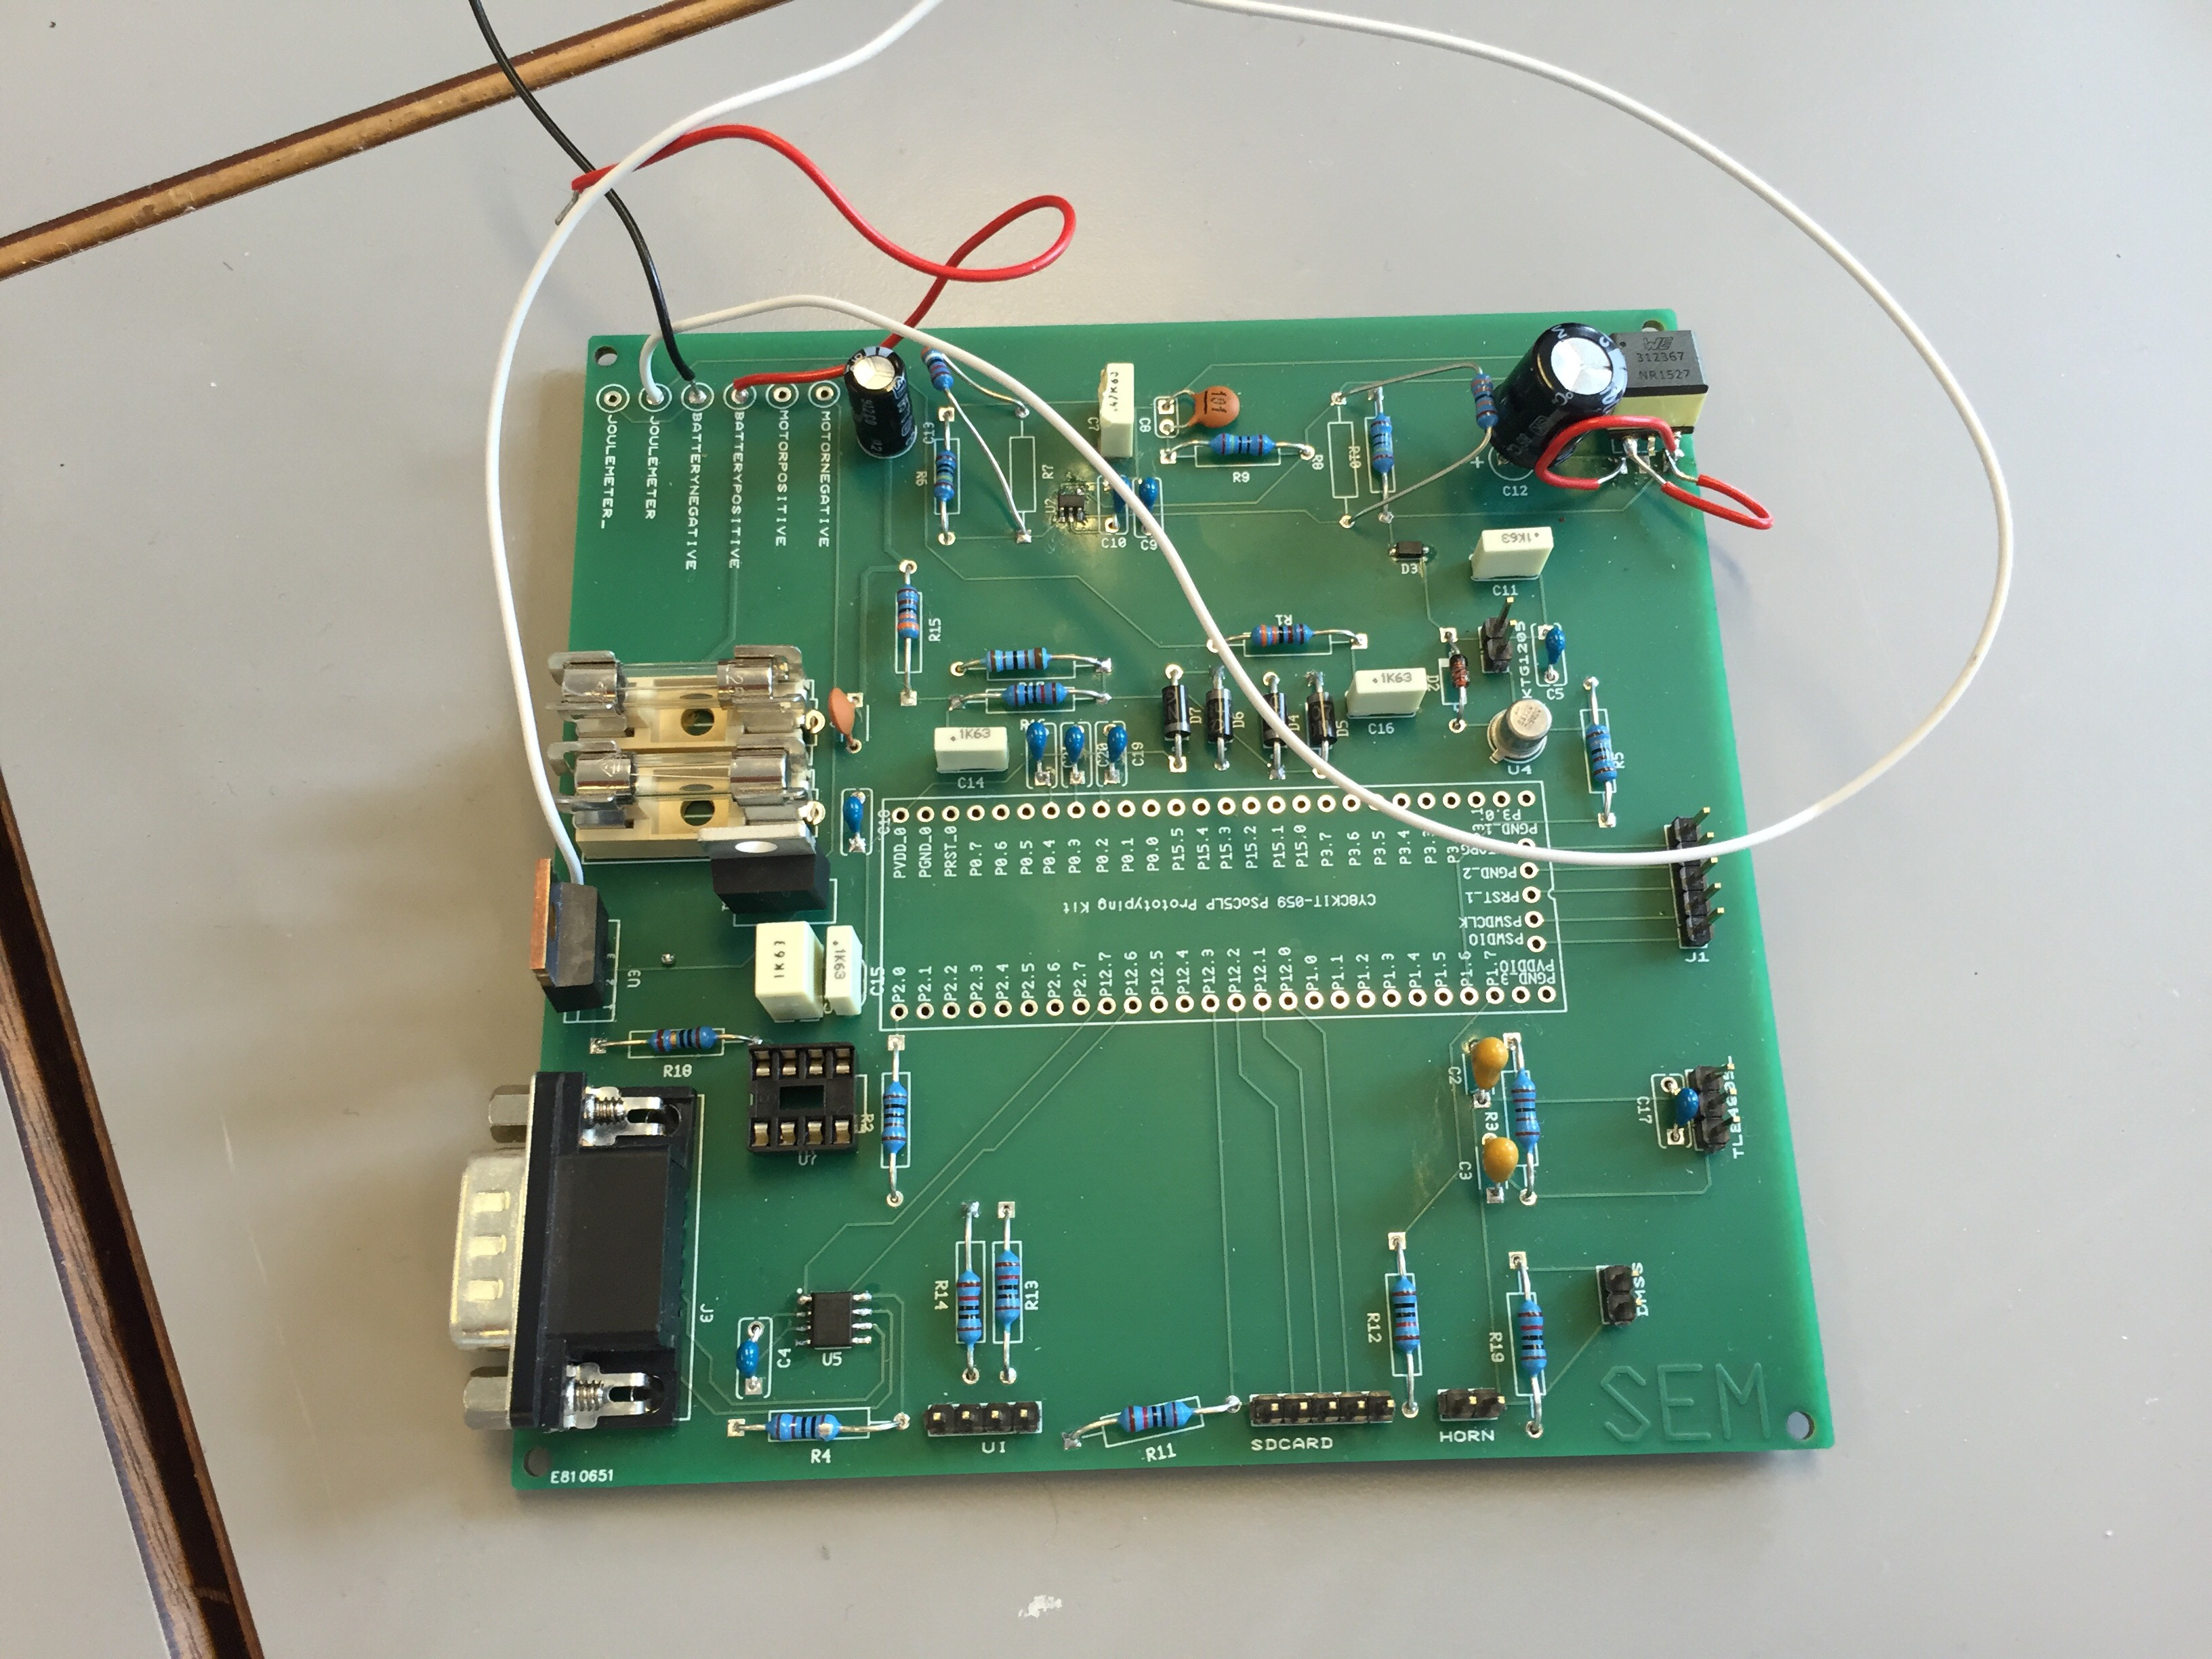
\includegraphics[width=0.6\linewidth]{SubPages/Images/SD_MCS}
	\caption{Motor control system}
	\label{fig:SD_MCS}
\end{figure}

The BMS(Battery management system) can be seen on figure \vref{fig:SD_BMS}, with the following components:

\begin{enumerate}
	\item Isolation Switch
	\item Digital Unit
	\item Digital Unit \fxnote{kan man lave de to i en samlet box, Jonas?}
	\item Analog Front End Extension Module(above) \& Analog Front End(under)
	\item Current sensor
	\item Batteries
	\item DC/DC Converter
\end{enumerate}

\begin{figure}[H]
	\centering
	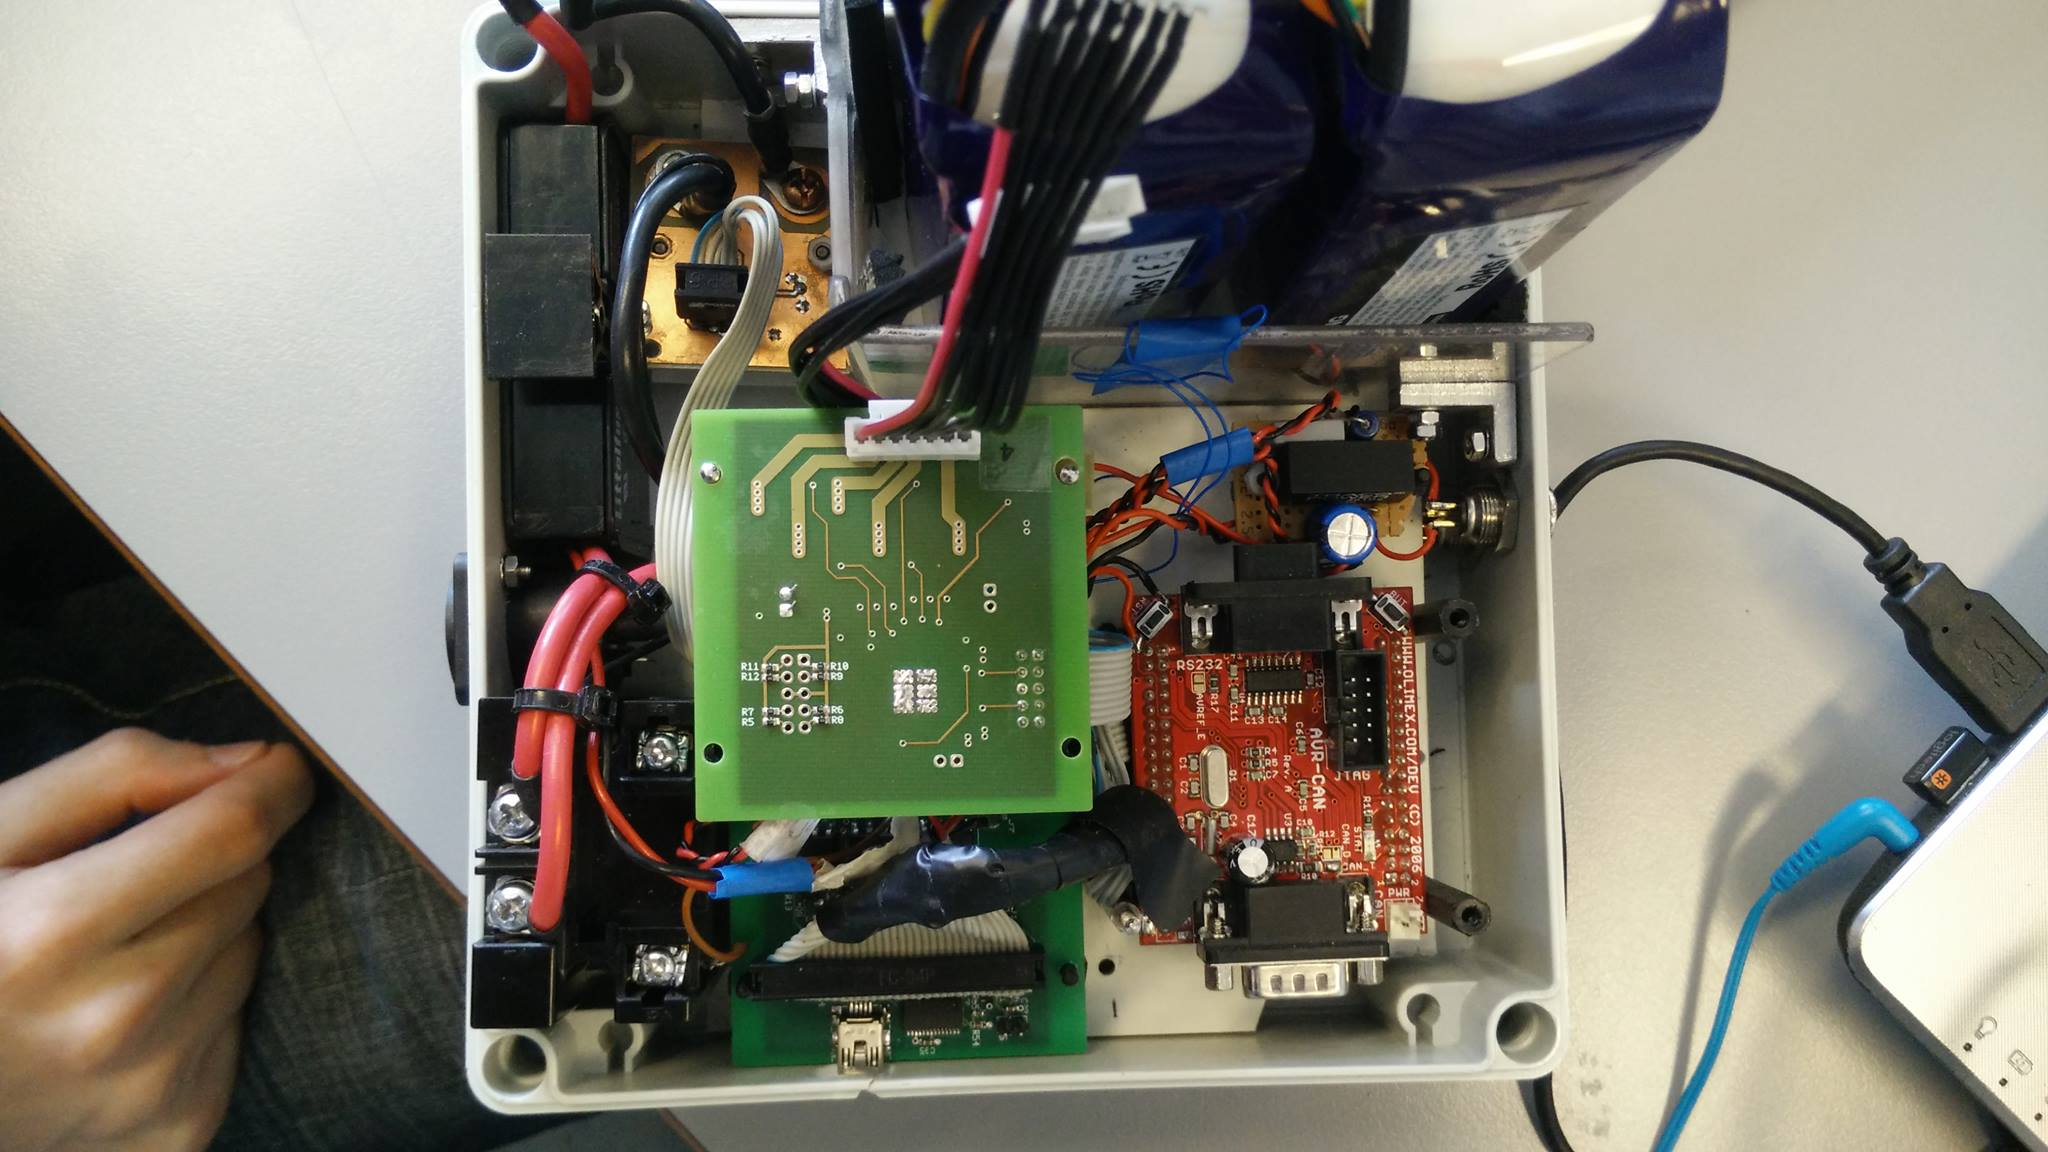
\includegraphics[width=0.7\linewidth]{SubPages/Images/SD_BMS}
	\caption{Battery management system}
	\label{fig:SD_BMS}
\end{figure}

\section{Rolling Road}
The Control-box containing the PCB and the PSoC can be seen in figure \vref{fig:SD_RR}. Around the edge of the box all external connections can be seen. These are color-coded banana-plugs for easy interconnectivity, a coax 2.1mm DC-plug for power-supply and a USB-port for the communication with the PSoC. 

\begin{figure}[H]
	\centering
	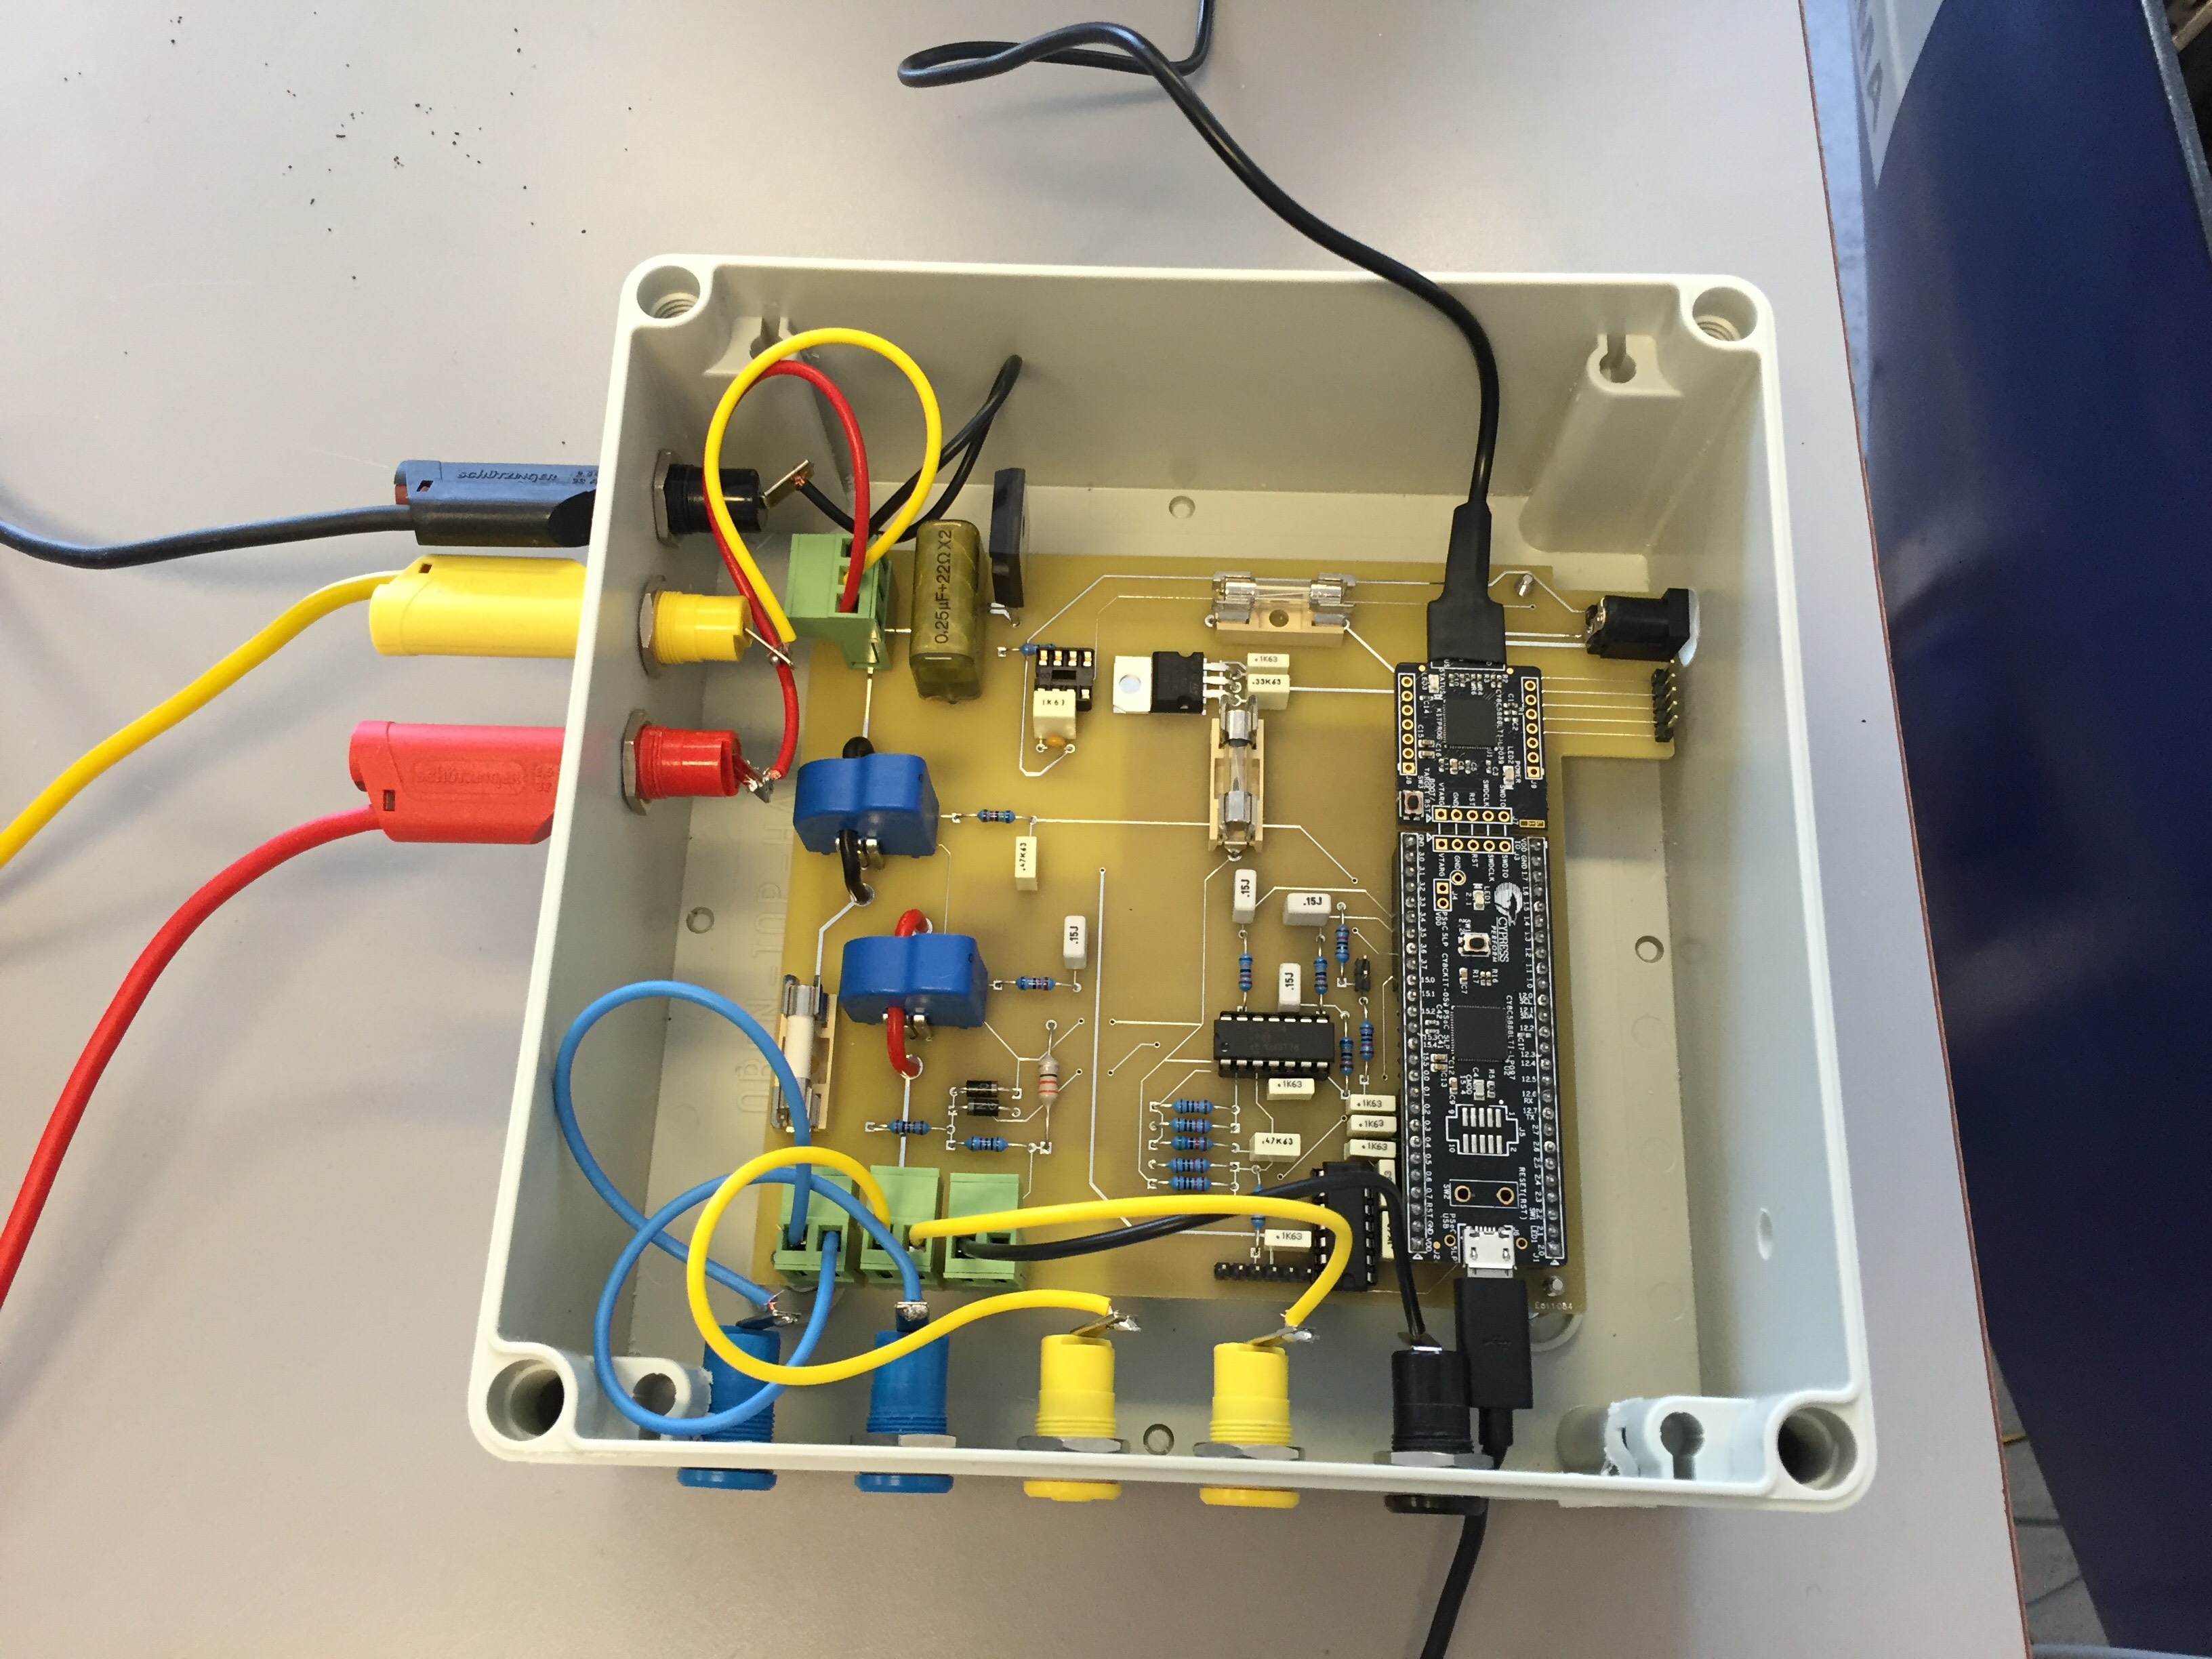
\includegraphics[width=0.7\linewidth]{SubPages/Images/SD_RR}
	\caption{Rolling Road Controller}
	\label{fig:SD_RR}
\end{figure}

\newpage
The Physical stand containing the Roll (left), the Generator (right) and the Torque Sensor (center) can be seen on figure \vref{fig:SS_RR_Roal}.

\begin{figure}[H]
	\centering
	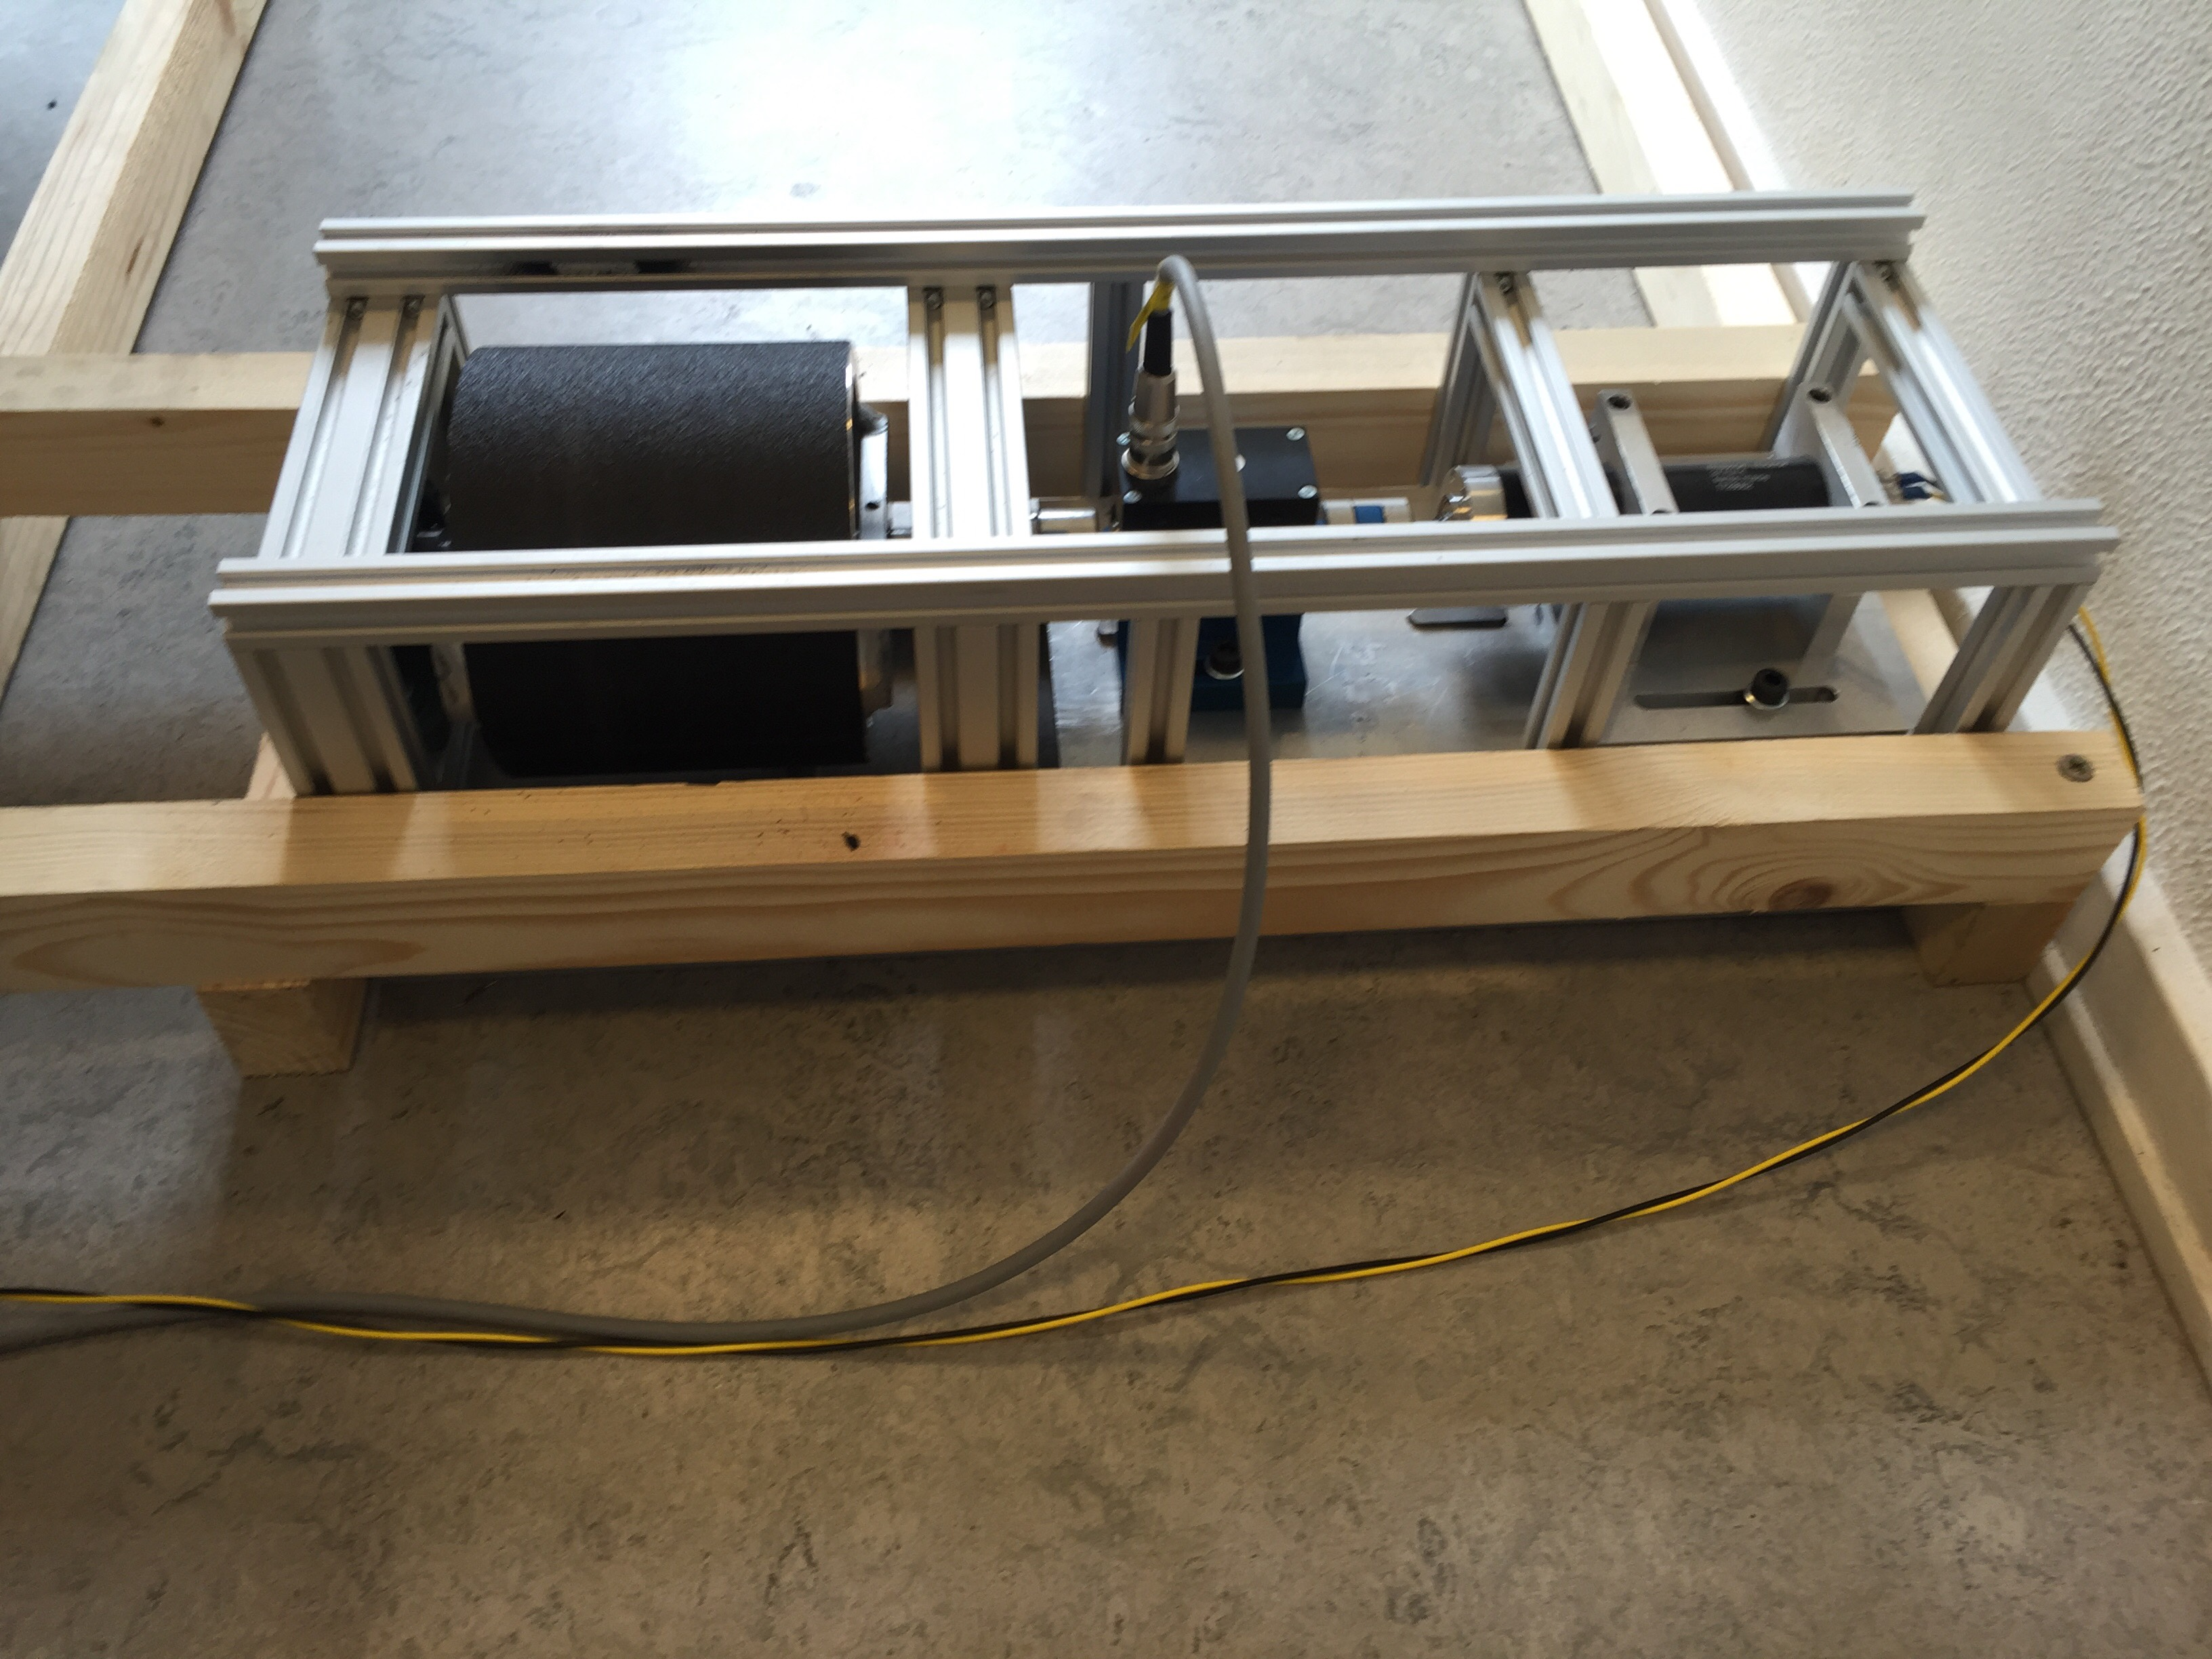
\includegraphics[width=0.7\linewidth]{SubPages/Images/SS_RR_Roal}
	\caption{Rolling Road}
	\label{fig:SS_RR_Roal}
\end{figure}

The Load-plate containing the super capacitor and the two power resistors can be seen on figure \vref{fig:SD_RR_Load}. This plate can be connected to the Control-box using the banana-plugs.

\begin{figure}[H]
	\centering
	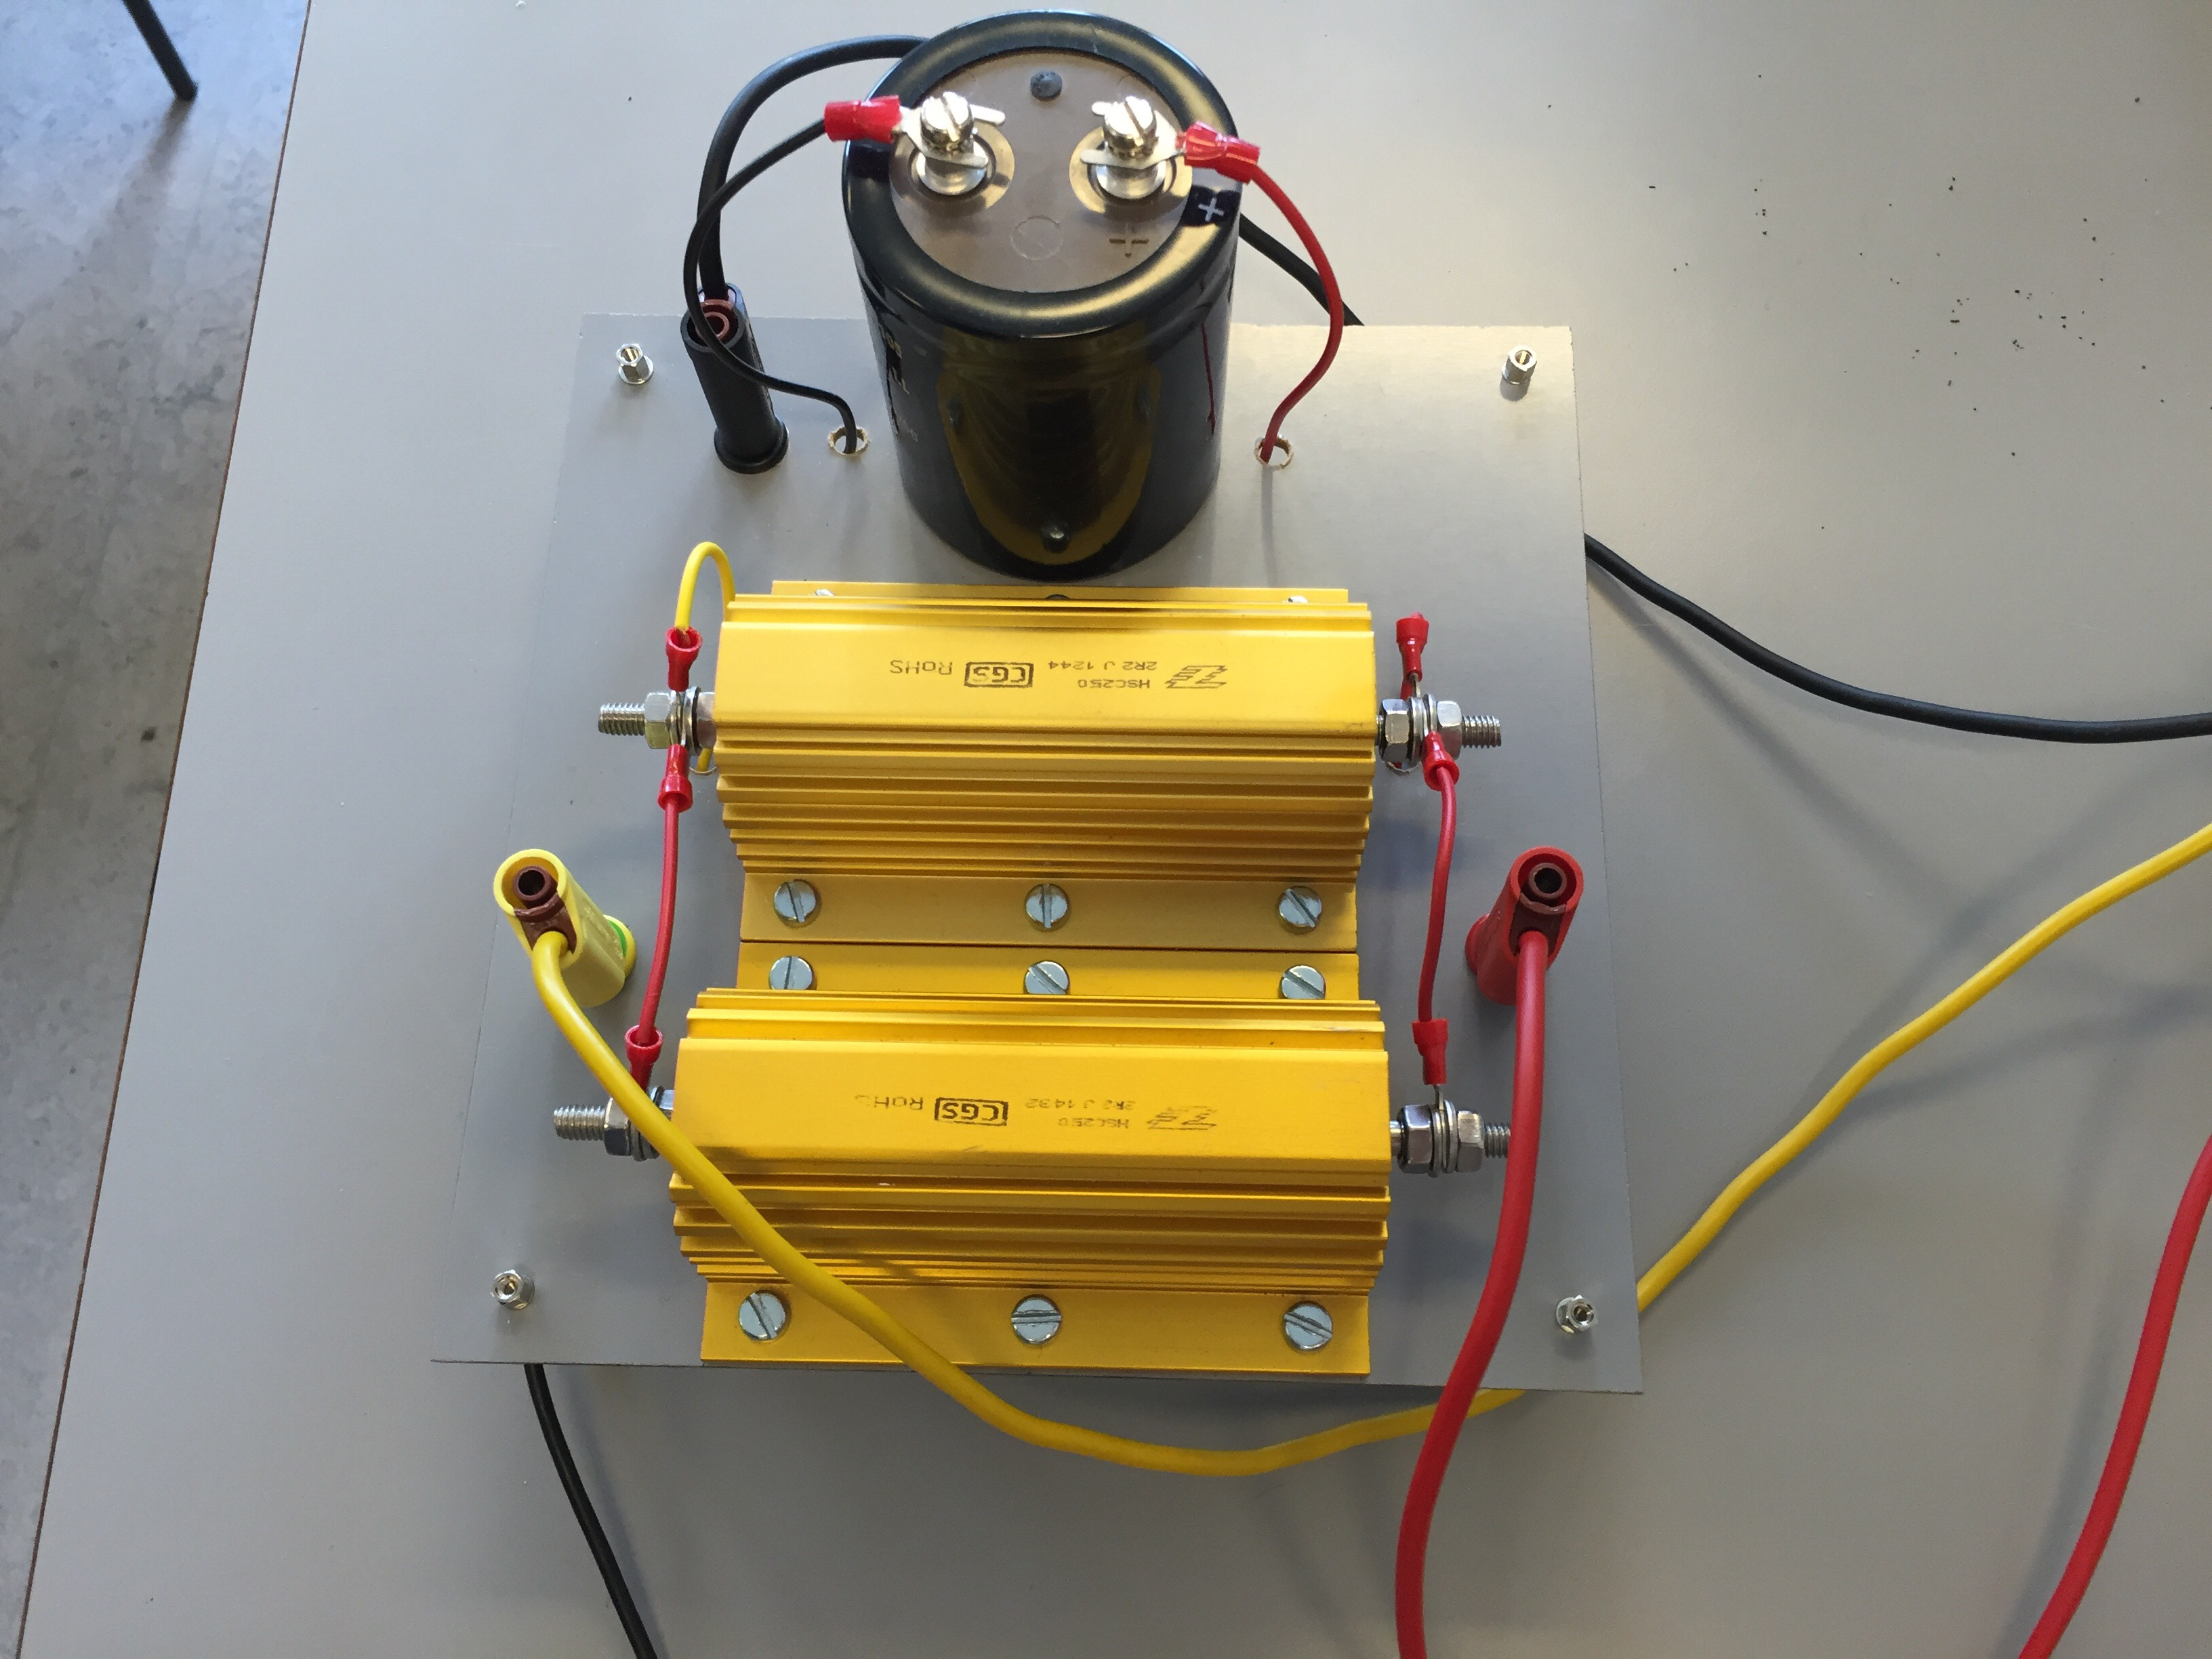
\includegraphics[width=0.7\linewidth]{SubPages/Images/SD_RR_Load}
	\caption{Load-plate}
	\label{fig:SD_RR_Load}
\end{figure}

\newpage
\section{Rolling Road GUI}
The Rolling Road live-data display, where simulated data has been collected and displayed to the user. To the left all the control would be available if connected to the Rolling Road, and to the right the latest readings from the Rolling Road can be seen.

\begin{figure}[H]
	\centering
	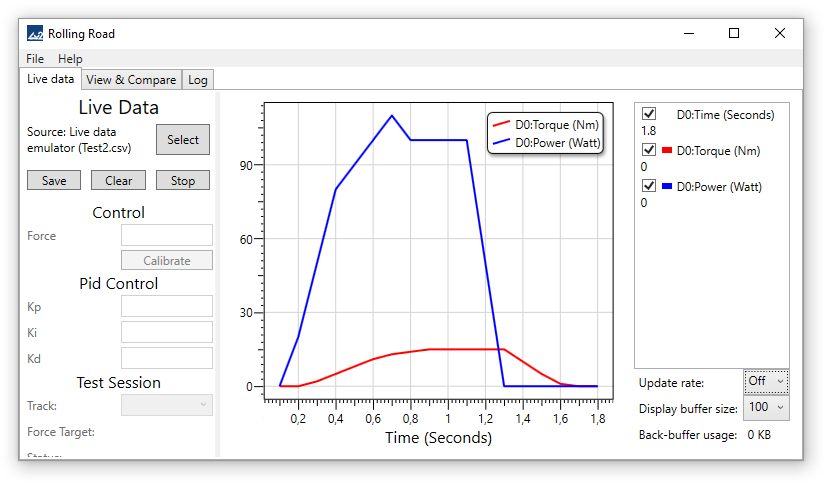
\includegraphics[width=0.9\linewidth]{SubPages/Images/SD_GUI}
	\caption{Rolling Road GUI}
	\label{fig:SD_GUI}
\end{figure}
